\chapter{Circular Motion}
\index{circular motion}
Let's say you tie a 0.16 kg billard ball to a long string and begin to swing
it around in a circle above your head. The string is 3
meters long, and the ball returns to where it started every 4
seconds. We will assume the ball moves at a constant speed. If you start your stopwatch as the ball crosses the
$x$-axis, the position of the ball at any time $t$ given by:

$$p(t) = [3 \cos{\left( \frac{2 \pi} {4}t\right)}, 3 \sin{ \left( \frac{2 \pi}{4}t\right) }, 2]$$

(This assumes that the ball would be going counter-clockwise if viewed
from above. The spot you are standing on is considered the origin $[0, 0, 0]$.)

Notice that the height is a constant --- 2 meters in this
case. That isn't very interesting, so we will talk just about the
first two components.  Here is what it would look like from above:

% 3sin = 1.267854785222098
% 3cos = 2.71892336110995

\begin{figure}[htbp]
    \begin{center}
        
        \begin{tikzpicture}[declare function={angle=25;},bullet/.style={inner
            sep=1pt,fill,draw,circle,solid}, scale=1.7]
            % Axis
            \draw[thick,-stealth,black] (-3.2,0)--(3.2,0) node[right] {$x$}; % x axis
            \draw[thick,-stealth,black] (0,-3.2)--(0,3.2) node[left] {$y$}; % y axis
            % Rest
            \draw [dashed, sdkblue] (0,0) circle (3);
            \draw[thick] (0,0) -- (angle:3.0) node [midway, above] {3};
            \draw[sdkblue] (1.05, 0.2) node[right] {$\theta = \frac{2\pi t}{4}\text{ radians}$};
            \draw[-stealth,sdkblue] (1,0) arc (0:angle:1);
            \draw[dashed, black] (2.71892336110995, 1.267854785222098) -- (2.71892336110995, 0)
            node[below] {$3 \cos(\theta)$}; % vertical
            \draw[dashed, black] (2.71892336110995, 1.267854785222098) -- (0, 1.267854785222098)
            node[left] {$3 \sin(\theta)$}; % horizontal
            \filldraw[black] (angle:3.0) circle(4pt);
            \draw[->, thick] (2.71892336110995, 1.267854785222098) --
            (2.71892336110995 - 3 * 0.1267, 1.267854785222098 + 3 * 0.2718);
        \end{tikzpicture}
    \end{center}
        \caption{A diagram of our ball and string scenario.}
    \label{fig:billiardBall}
\end{figure}

In this case, the radius, $r$, is 3 meters.  The period, $T$, is 4
seconds.  In general, we say that circular motion is given by:

$$p(t) = \left[ r \cos{\frac{2 \pi t}{T}}, r \cos{\frac{2 \pi t}{T}}\right]$$

A common question is ``How fast is it turning right now?''  If you
divide the $2\pi$ radians of a circle by the 4 seconds it takes, you
get the answer ``About 1.57 radians per second.''  This is known as
\newterm{angular velocity} and we typically represent it with the
lowercase Omega: $\omega$. (Yes, it looks a lot like a ``w''.)  To be
precise, in our example, the angular velocity is $\omega = \frac{\pi}{2}$. Note that in this scenario, the angular velocity and linear \emph{speed} are constant. However, the \emph{velocity} vector is not constant; as we will see in the next section, the direction of the velocity vector is always changing.

Notice that this is different from the question ``How fast is it
going? (referring to \newterm{linear velocity})''  This ball is traveling the circumference of $6\pi \approx
18.85$ meters every 4 seconds.  This means the speed of the ball is about
4.71 meters per second.

It is very important to distinguish between angular velocity and linear velocity. Angular velocity is how fast the angle is changing and is referred to by $\omega$, while linear velocity, $v$, is how fast the object is moving along its path. While linear velocity has a constant speed, it has always changing direction. The angular velocity is constant, but the linear velocity is not.

\section{Velocity}
\index{circular motion ! velocity}
The velocity of the ball is a vector, and we can find that vector by
differentiating each component of the position vector.

For any constants $a$ and $b$:

\begin{tabular}{c | c }
  Expression & Derivative \\
  \hline
  $a \sin{b t}$ & $ab \cos{b t}$ \\
  $a \cos{b t}$ & $-ab \sin{b t}$  \\
\end{tabular}

Thus, in our example, the velocity of the ball at any time $t$ is given by:

$$v(t) = \left[ -\frac{3 (2\pi)}{4} \sin{\frac{2\pi t}{4}}, \frac{3(2\pi)}{4} \cos{\frac{2\pi t}{4}}, 0 \right]$$

Notice that the velocity vector is perpendicular to the position vector.  It has a constant magnitude.

In general, an object traveling in a circle at a constant speed has the velocity vector:

$$v(t) = \left[ -r\omega \sin{\omega t}, r\omega \cos{\omega t}\right]$$

where $t = 0$ is the time that it crosses the $x$ axis.  If $\omega$ is
negative, that means the motion would be clockwise when viewed from
above.

The magnitude of the velocity vector is $r\omega$. 
\begin{figure}[htbp]
\begin{center}
    
        \begin{tikzpicture}[declare function={angle=25;},bullet/.style={inner
            sep=1pt,fill,draw,circle,solid}, scale=1.7]
            % Axis
            \draw[thick,-stealth,black] (-3.2,0)--(3.2,0) node[right] {$x$}; % x axis
            \draw[thick,-stealth,black] (0,-3.2)--(0,3.2) node[left] {$y$}; % y axis
            % Rest
            \draw [dashed, sdkblue] (0,0) circle (3);
            \filldraw[black] (angle:3.0) circle(4pt);
            \draw[->, thick] (2.71892336110995, 1.267854785222098) --
            (2.71892336110995 - 0.6 * 1.267, 1.267854785222098 + 0.6 * 2.718) node[right]{$v(t)=\left[ -r\omega \sin{\omega t}, r\omega \cos{\omega t}\right]$};
        \end{tikzpicture}
    
\end{center}    \caption{Velocity vector of the ball in circular motion.}
    \label{fig:billardBallVelocity}
\end{figure}

\begin{Exercise}[title = {A Particle in Motion}, label = particle]
[This question was originally presented as two multiple-choice problems on the 2012 AP Physics C exam.] The $x$ and $y$ coordinates of a particle as it moves in a circle are given by:
$$x = 5\cos{\left( 3t \right)}\\
y = 5\sin{\left( 3t \right)}$$

What is the radius of the particle's circular path? What is the particle's \textit{speed}? Based on your answers, how long does it take the particle to complete the circular path?
\vspace{50mm}
\end{Exercise}

\begin{Answer}[ref = particle]
The radius is 5 m, because the coefficients of both the $x$ and $y$ functions is 5. 

Recall that the velocity in each direction is given by the derivative of the position functions:
$$v_x(t) = \frac{d}{dt} \left[ 5 \cos{ \left( 3t \right)} \right] = -15 \sin{ \left( 3t \right)}$$
$$v_y(t) = \frac{d}{dt} \left[ 5 \sin{ \left( 3t \right)} \right] = 15 \cos{ \left( 3t \right)}$$

The overall \textit{speed} can be found from the $x$ and $y$ components of the velocity:
$$|v| = \sqrt{v_x^2 + v_y^2} = \sqrt{\left[ -15 \sin{ \left( 3t \right) } \right]^2 + \left[ 15 \cos{ \left( 3t \right)} \right]^2}$$
$$|v| = \sqrt{15^2 \left[ \sin{ \left(3t \right)}^2 + \cos{ \left( 3t \right)}^2 \right]} = \sqrt{15^2} = 15 \frac{m}{s}$$

Notice that this is the coefficient for both components of the velocity. 

To complete the path, the particle must travel $10\pi \text{ } m$. If the speed is $15 \frac{m}{s}$, then the time it takes is:
$$t = \frac{d}{v} = \frac{10\pi \text{ } m}{15 \frac{m}{s}} = \frac{2\pi}{3} s \approx 2.09 \text{ } s$$
\end{Answer}

\section{Acceleration}

We can get the (linear) acceleration by differentiating the components of the velocity vector.

$$a(t) = \left[-r \omega^2 \cos{\omega t}, -r \omega^2 \sin{\omega t} \right]$$

Notice that the acceleration vector points \textbf{toward the center} of the
circle it is traveling on. That is, when an object is traveling on a
circle at a constant speed (notice that the coefficients in $a(t)$ are constant values, so acceleration is constant), its only acceleration is toward the center of the circle. This is known as \newterm{centripetal acceleration}. \index{centripetal ! acceleration}

\begin{figure}[htbp]
    \begin{center}
        
        \begin{tikzpicture}[declare function={angle=25;},bullet/.style={inner
            sep=1pt,fill,draw,circle,solid}, scale=1.7]
            % Axis
            \draw[thick,-stealth,black] (-3.2,0)--(3.2,0) node[right] {$x$}; % x axis
            \draw[thick,-stealth,black] (0,-3.2)--(0,3.2) node[left] {$y$}; % y axis
            % Rest
            \draw [dashed, sdkblue] (0,0) circle (3);
            \filldraw[black] (angle:3.0) circle(4pt);
            \draw[->, thick] (2.71892336110995, 1.267854785222098) --
            (2.71892336110995 * 0.2 , 1.267854785222098 * 0.2) node[midway, right]{$a(t) = \left[-r \omega^2 \cos{\omega t}, -r \omega^2 \sin{\omega t} \right]$};
        \end{tikzpicture}
    \end{center}
    \caption{Acceleration vector of the particle in circular motion.}
    \label{fig:billardBallAcceleration}
\end{figure}

The magnitude of the acceleration vector is $r \omega^2$.

\section{Centripetal force}

How hard is the ball pulling against your hand? That is, if you let go, the ball would fly in a straight line.  
The force you are exerting on the string is what causes it to accelerate toward the center of the
circle. We call this the \newterm{centripetal force}. It makes sense that the centripetal force and centripetal acceleration are in the same direction. \index{centripetal ! force}

Recall that $F = m a$.  The magnitude of the acceleration is $r
\omega^2 = 3 \left(\frac{2 pi}{4}\right)^2 \approx 7.4$ m/s/s.  The mass
of the ball is 0.16 kg.  So, the force pulling against your hand is
about 1.18 newtons.

The general rule is that when something is traveling in a circle at a
constant speed, the centripetal force needed to keep it traveling in a
circle is:

$$F = m r \omega^2$$

If you know the radius $r$ and the speed $v$ of the object, here is the rule:

$$F = \frac{m v^2}{r}$$

We didn't introduce centripetal force as a type of force because it isn't its own force, like friction or gravity. Rather, calling a force "centripetal" tells us what the force is doing. A centripetal force is any force that causes circular motion. For a satellite, the centripetal force is gravity. In the opening example with the billiard ball, the centripetal force is the tension in the string. 

\textbf{Example}: A child is sitting on a merry-go-round as it spins. What provides the centripetal force? 

\textbf{Solution}: In this case, the child is rotating horizontally, so the centripetal force must also be horizontal. Therefore, the centripetal force isn't the child's weight or the normal force. It is the \textit{friction} between the child and the merry-go-round that keeps the child turning. Here is a free body diagram:

%FBD child merry-go-round fixme

\textbf{Example}: If the child is 1.2 meters from the center of the merry-go-round and it spins at 0.25 rotations/second, what is the coefficient of friction between the child and the merry-go-round?

\textbf{Solution}: Using our FBD and applying Newton's Second Law, we see that:
$$F_N - F_g = 0 \to F_N = m_{child}g$$
$$F_f = m r \omega^2 = \mu F_N = \mu m g$$

Since the child isn't accelerating vertically, we know that the normal force equals the child's weight. The horizontal force, friction, must equal the mass of the child times the acceleration. Additionally, from the vertical component, we know the friction is equal to $\mu m g$, since the normal force is equal to the child's weight. Looking at the second equation, we see that:
$$m r \omega^2 = \mu m g$$

We were given $\omega$ in rotations per second, but we need radians per second:
$$\frac{0.25 \text{rotation}}{1 \text{second}} = \frac{1 \text{rotation}}{4 \text{seconds}} = \frac{2\pi \text{radians}}{4 \text{seconds}} = \frac{\pi}{2} \frac{rad}{s}$$
We can divide $m$ from both sides of $mr\omega^2 = \mu m g$ (notice: we don't need to know the child's mass to determine the coefficient of friction!):
$$r \omega^2 = \mu g \to \mu = \frac{r \omega^2}{g} = \frac{\left( 1.2 m \right) \left( \frac{\pi}{2 s} \right)^2}{9.8 \frac{m}{s^2}} = 0.302$$

Therefore, the coefficient of friction between the child and the merry-go-round is 0.302. 

\subsection{Banked Turns}
Have you every been driving on the highway and taken a turn where the road is at an angle? Or maybe you've seen a sign like this on the road:

\begin{wrapfigure}{r}{2.5in}
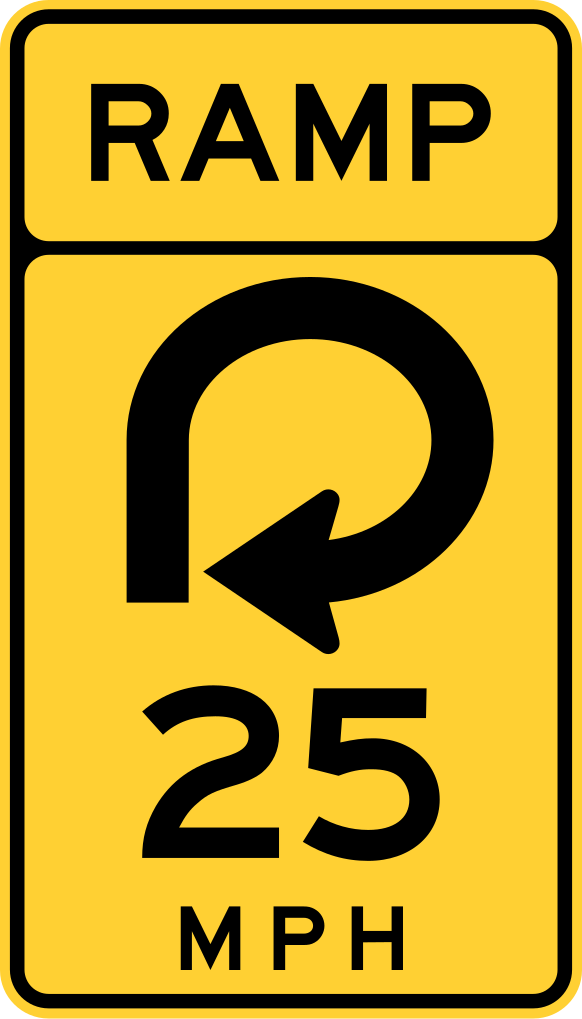
\includegraphics[width=2.5in]{traffic.png}
\end{wrapfigure}

A banked curve is designed so that a car can safely turn without slipping, even in the rain, if the driver does not exceed the indicated speed. Engineers choose an angle such that the bank provides sufficient force to turn the car without friction. Let's look at a free body diagram for a car taking a banked turn (see figure \ref{fig:banked}). 
\vspace{4cm} %FIXME formatting
\begin{figure}[htbp]
    \centering
    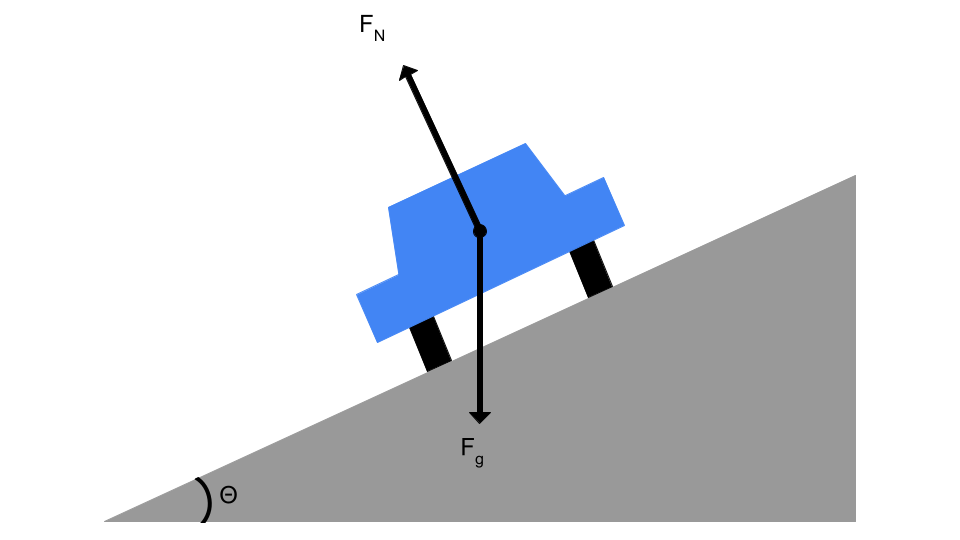
\includegraphics[width=4in]{banked.png}
    \caption{If there is no friction due to rain, then the only two forces acting on the car are gravity and the normal force.}
    \label{fig:banked}
\end{figure}

In the past, we've split the vector for the force of gravity into components that are parallel and perpendicular to the ramp. This time, we will split the normal force into $x$ and $y$ components (see figure \ref{fig:banked_component}). 

\begin{figure}[htbp]
\centering
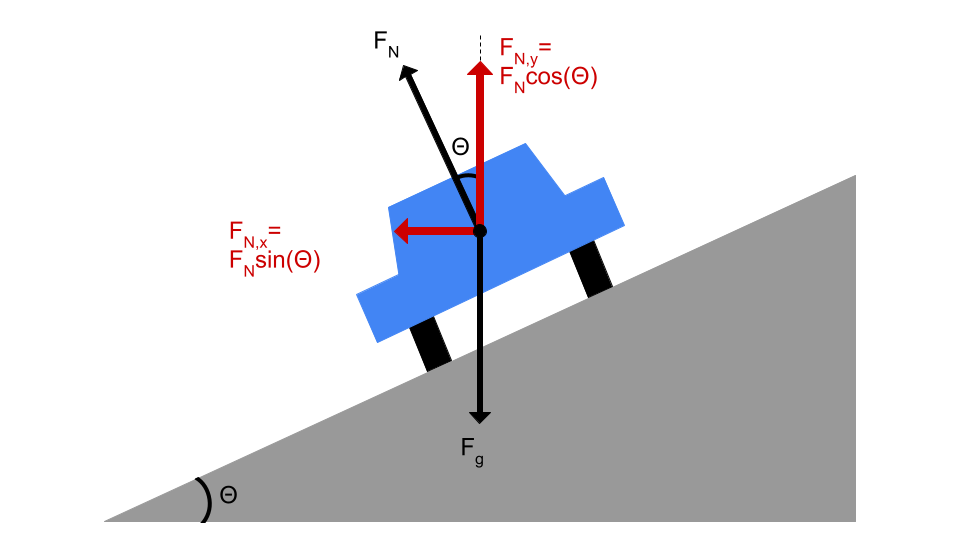
\includegraphics[width=4in]{banked_component.png}
\caption{Geometrically, the $x$ component of the normal force is given by $F_N \cos{\left( \theta \right)}$ and the $y$ component by $F_N \sin{ \left( \theta \right)}$.}
\label{fig:banked_component}
\end{figure}

Assuming the radius of the turn is 20 m, at what angle should the engineers build the banked turn? (Let's also assume the maximum speed is 25 mph, like the traffic sign above.) First, let's apply Newton's Second Law in the $x$ and $y$ directions:
$$\left( 1 \right) F_N \cos{ \left( \theta \right) } - F_g = 0$$
$$\left( 2 \right) F_N \sin{ \left( \theta \right) } = \frac{mv^2}{r}$$

We know that $F_g = mg$. From this and equation (1) we see that:
$$F_N = \frac{mg}{\cos{ \left( \theta \right)}}$$

Substituting for $F_N$ into equation (2):
$$\left( \frac{mg}{\cos{ \left( \theta \right)}} \right) \sin{ \left( \theta \right)} = \frac{mv^2}{r}$$

The mass can be divided from both sides, and $\frac{\sin{ \left( \theta \right)}}{\cos{ \left( \theta \right)}} = \tan{ \left( \theta \right)}$:
$$g \tan{ \left( \theta \right)} = \frac{v^2}{r}$$

Solving for $\theta$ and substituting for the speed ($25 \text{ }mph \approx 11.18 \frac{m}{s}$) and radius:
$$\theta = \arctan{ \left( \frac{v^2}{gr} \right)} = \arctan{ \left( \frac{\left( 11.18 \frac{m}{s} \right)^2}{\left( 9.8 \frac{m}{s^2} \right) \left( 20 m \right)} \right)}$$
$$\theta = \arctan{ \left( 0.6377 \right) } \approx 32.53 ^{\circ}$$


\section{Modeling Circular Motion}
What causes circular motion is a constant force perpendicular to the motion. Consider a satellite circling the Earth. The only force acting on the satellite is gravity, yet the satellite does not fall to the Earth. Why? Let's look at the relative direction of motion and gravity for some different positions of the satellite (we'll assume this satellite is moving clockwise from our point of view):

\begin{center}
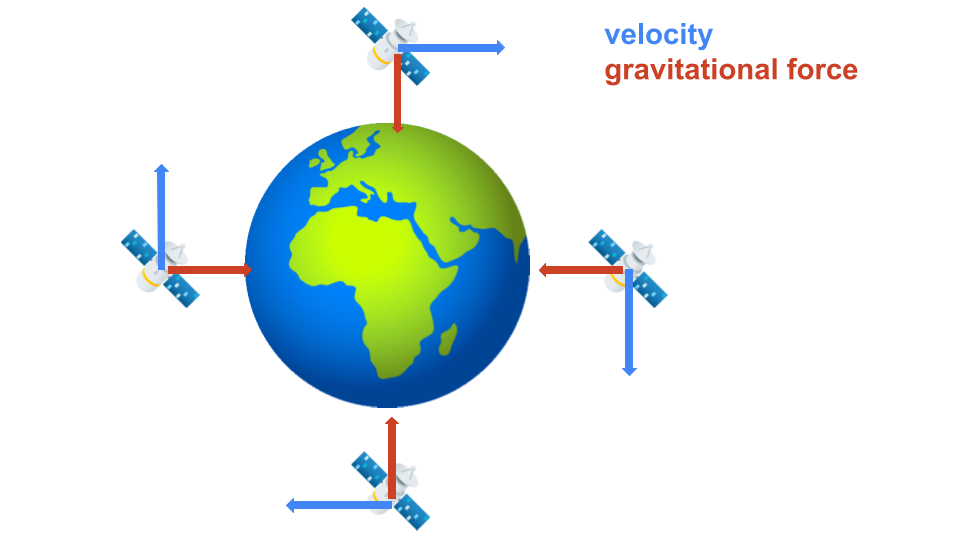
\includegraphics[width=4in]{satellite.png}
\end{center}

No matter what position the satellite is in, the velocity and gravity vectors are perpendicular. 

%fix me: section discussing work and delta KE, perpendicular, dot product, no change in v

\begin{Exercise}[title={Circular Motion}, label=circular]
Just as your car rolls onto a circular track with a radius of 200 m,
you realize your 0.4 kg cup of coffee is on the slippery dashboard of your
car.  While driving 120 km/hour, you hold the cup to keep it from sliding.

What is the maximum amount of force you would need to use? (The friction of
the dashboard helps you, but the max is when the friction is zero.)

\end{Exercise}
\begin{Answer}[ref=circular]
  $$\frac{120 \text{ km}}{1 hour} = \frac{1000 \text{ m}}{1 \text{ km}}\frac{120 \text{ km}}{1 hour} \frac{1 \text{ hour}}{3600 \text{ seconds}}= 33.3 \text{ m/s}$$

  $$F = \frac{m v^2}{r} = \frac {0.4 (33.3)^2}{200} = 2.2 \text{ newtons}$$
\end{Answer}

\begin{Exercise}[title = {Twirling a Whistle}, label = whistle]
The lifeguard at a local pool is twirling their whistle horizontally. You wonder if the lifeguard could spin the whistle fast enough to break the string. The string the whistle is attached to can hold a maximum mass of 20 kg before breaking. If the lifeguard's whistle string is 0.35 m long and the average whistle has a mass of 165 grams, what is the maximum tangential speed the lifeguard can spin the whistle? How many rotations per second would the whistle be spinning at? Based on this, do you think the lifeguard is capable of spinning the whistle fast enough to break the string?
\end{Exercise}

\begin{Answer}[ref = whistle]
Givens:
$$T_{max} = \left( 20 kg \right) \cdot \left( 9.8 \frac{m}{s^2} \right) = 196 N$$
$$r = 0.35 m$$
$$m_{whistle} = 165 g = 0.165 kg$$

Unknown:
$$v = ?$$
$$f = ?$$

Equation(s):
$$F = ma$$
$$a = \frac{v^2}{r}$$
$$v = rf$$

Solution:
First, we find the tangential speed if the tension in the string is the maximum tension:
$$T_{max} = m_{whistle}a = m_{whistle} \frac{v^2}{r}$$
$$v = \sqrt{\frac{T_{max}r}{m_{whistle}}}$$
$$v = \sqrt{\frac{196 N \left(0.35 m \right)}{0.165 kg}} \approx 0.645 \frac{m}{s}$$

Therefore, the maximum tangential speed of the whistle before the string breaks is $0.645 \frac{m}{s}$. Now finding the equivalent frequency (rotations per second):
$$f = \frac{v}{r} = \frac{0.645 \frac{m}{s}}{0.35 m} \approx 1.842 Hz$$

So, to break the string, the lifeguard would have to spin it at nearly 2 rotations per second, which is achievable. The lifeguard could possibly break the string. 
\end{Answer}

\begin{Exercise}[title = {The Gravitron}, label = gravitron]
The Gravitron is a carnival ride where riders "stick" to the wall of a spinning cylinder as the floor beneath them drops away. A video explanation is given here: \url{https://www.youtube.com/watch?v=ifAY5tbYDmQ}. Draw a free body diagram of a rider. If the coefficient of friction between a rider and the wall is 0.32 and the ride is 10 meters across, what angular velocity must the ride reach before the floor drops away?
\end{Exercise}

\begin{Answer}[ref = gravitron]
There are three forces acting on the rider: gravity, friction with the wall, and the normal force with the wall:

\begin{center}
    \begin{tikzpicture}
        \draw[thick] (-1, -1) rectangle (1,1);
        \draw[fill=black] (0,0) circle (0.5mm);
        \draw[-latex] (0,0) -- (0, 2) node[above] {$F_f$};
        \draw[-latex] (0,0) -- (3, 0) node[right] {$F_N$};
        \draw[-latex] (0,0) -- (0, -2) node[below] {$F_g$};
    \end{tikzpicture}
\end{center}

The FBD lets us write equations for Newton's Second Law in each dimension:
$$\left( 1 \right) \text{ }ma_x = F_N$$
$$\left( 2 \right) \text{ }ma_y = F_f - F_g = \mu F_N - mg$$

Because the rider doesn't fall down, we know that $a_y = 0 \frac{m}{s^2}$ and therefore equation (2) becomes:
$$\mu F_N - mg = 0 \to F_N = \frac{mg}{\mu}$$

Having solved for $F_N$, we substitute for it into equation (1):
$$ma_x = \frac{mg}{\mu} \to a_x = \frac{g}{\mu}$$

Since we know $g$ and $\mu$, we can calculate $a_x$:
$$a_x = \frac{9.8 \frac{m}{s^2}}{0.32} = 30.625 \frac{m}{s^2}$$

This is the minimum acceleration needed to keep the rider from slipping down. We can now use the relationship between centripetal acceleration, tangential velocity, and the radius to find the angular velocity:
$$a = \frac{v^2}{r} = \frac{\left( \omega r \right)^2}{r} = \omega^2 r$$
$$\omega = \sqrt{\frac{a}{r}} = \sqrt{\frac{30.625 \frac{m}{s^2}}{10 \text{ } m}} \approx 1.75 \frac{rad}{s}$$
\end{Answer}

\section{Equations of Circular Motion}
\index{circular motion ! equations}
The same kinematic formulas can be used for circular motion, provided you use the correct variables. The angular displacement, $\theta$, is the angle in \emph{radians} that the object has traveled. The angular velocity, $\omega$, is the rate of change of the angular displacement, and the angular acceleration, $\alpha$, is the rate of change of the angular velocity.

\begin{center}
    \begin{align}
      v &= v_0 + a t 
      &\qquad\qquad&
      \omega \;=\; \omega_0 + \alpha t \\[4pt]
      x &= x_0 + v_0 t + \tfrac12 a t^{2} 
      &&
      \theta \;=\; \theta_0 + \omega_0 t + \tfrac12 \alpha t^{2} \\[4pt]
      v^{2} &= v_0^{2} + 2a\!\left(x - x_0\right) 
      &&
      \omega^{2} \;=\; \omega_0^{2} + 2\alpha\!\left(\theta - \theta_0\right)
    \end{align}
\end{center}

Linear velocity, $v$, is related to angular velocity by the equation:
$$v = r \omega$$    

Period, $T$, is the time it takes to complete one full rotation. The frequency, $f$, is the number of rotations per second. The two are related by:
$$T = \frac{2\pi}{\omega} = \frac{2\pi r}{v}$$
$$f = \frac{1}{T}$$

The centripetal force, usually labelled differently (such as tension or gravity), is given by the equation:
$$F = m r \omega^2 = \frac{m v^2}{r}$$


The angular velocity, $\omega$ is rotations with respect to time. It can be defined in the following ways:
\[
  {\omega_{\text{inst}} = \frac{d\theta}{dt}}
  \qquad
  {\omega_{\text{avg}} = \frac{\Delta\theta}{\Delta t}}
\]

\[
  {\omega = 2\pi f = \frac{2\pi}{T} = \omega = \frac{v}{r}}
\]

Angular acceleration:
\[
\alpha = \frac{d\omega}{dt}, \qquad
\alpha_{\text{avg}} = \frac{\Delta\omega}{\Delta t}
\]